%%%%%%%%%%%%%%%%%%%%%%%%%%%%%%

\section{Overview of related work}

\begin{figure}
\centering
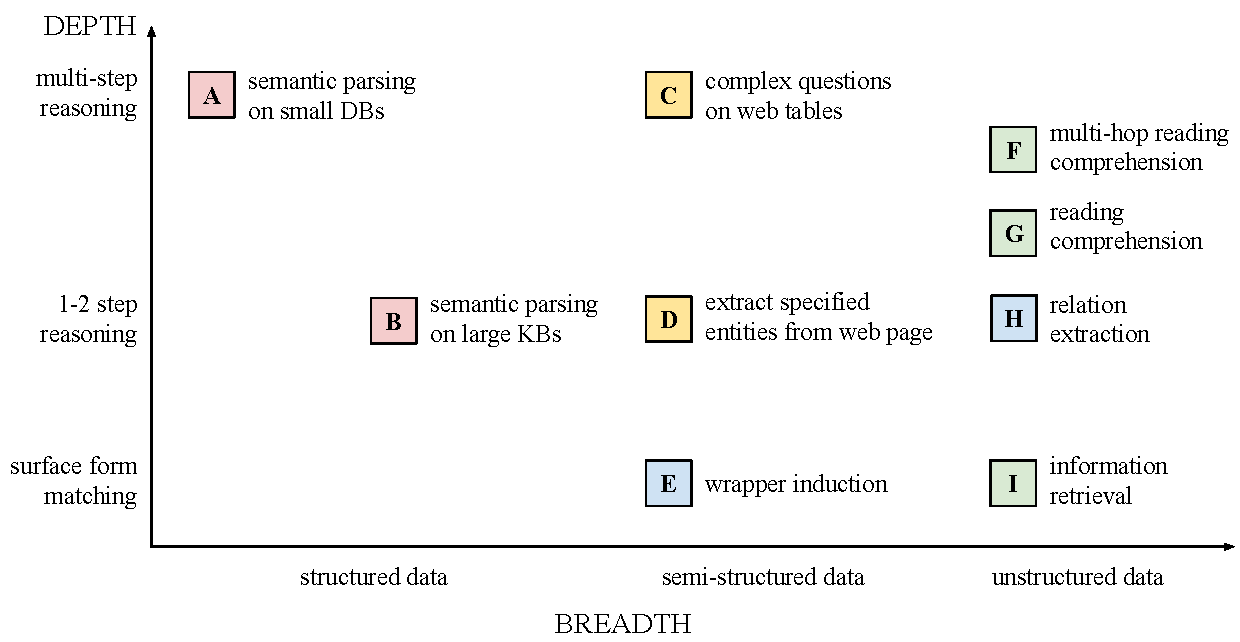
\includegraphics[width=\textwidth]{figures/intro/breadth-depth.pdf}
\caption
[Comparison of related work in terms of \Breadth and \Depth]
{Comparison of related work in two axes:
the scope of the domain (\Breadth)
and the complexity of the task (\Depth).
This dissertation starts
with exploring semi-structured data
(Point~D),
and then progresses to a task that addresses
both \Breadth and \Depth
simultaneously (Point~C).}
\label{fig:depth-breadth-plot}
\end{figure}

Figure~\ref{fig:depth-breadth-plot}
gives a broad picture of how our tasks and systems
situate among similar work in the
natural language processing literature.
While artificial intelligence was originally motivated
by tasks with very high \Depth and \Breadth
(Point~F),
such as the Turing test
\cite{turing1950computing},
it became evident that attacking two axes at once
was too challenging
for the technologies in that era.
Between the two axes,
several of the earlier works in artificial intelligence chose
to focus on \Depth:
they see the ability to perform complex reasoning
as the distinguishing trait of human's intelligence.
For natural language processing,
this results in systems that can handle very complex
utterances in a small fixed environment
(Point~A).
One prominent example is
SHRDLU \cite{winograd1972language},
a system that takes natural language commands,
manipulates blocks in a simulated
three-dimensional environment,
and generates natural language responses.
SHRDLU can understand complex, ambiguous,
and context-dependent utterances
while also performing spatial reasoning on the environment.
However, as a rule-based system,
it is brittle and cannot generalize to
linguistic variations or other environments.
This line of works on understanding very complex utterances
continues to evolve into the field
of semantic parsing,
which we discuss in more detail in
Section~\ref{sec:intro-semantic-parsing}.

In parallel, other early works
consider tasks in open-domain settings.
These works usually depend on
a shallow understanding of the utterance,
such as the surface forms of the strings,
token-level linguistic properties (e.g., part-of-speech
or named entity tags),
or subtree patterns of a syntactic tree.
For instance,
one classic broad-domain counterpart of SHRDLU is
ELIZA \cite{weizenbaum1966eliza},
a conversational agent
which uses generic but shallow sentence transformation rules
to generate replies based on the input utterances.
Other examples of open-domain tasks include
document retrieval (Point~J),
which mainly utilizes the surface forms of the strings
to rank the documents \cite{robertson2009probabilistic};
and information extraction
from semi-structured data (Point~E)
or unstructured data (Point~I),
which usually depends on patterns in
surface forms and
token-level syntactic tags \cite{hearst1992automatic,agichtein2000snowball},
syntactic parses \cite{mintz2009distant},
or other structural information
in the environment \cite{kushmerick1997wrapper,muslea2001hierarchical,arasu2003extracting}.
More recently, researchers have been
adding linguistic and functional complexity to
such open-domain tasks,
and using surface forms or patterns is no longer sufficient.
We discuss this progression in more detail
in Section~\ref{sec:intro-open-domain}.

\subsection{Executable semantic parsing}
\label{sec:intro-semantic-parsing}

Semantic parsing is the task of mapping
natural language utterance to its
meaning representation.
As different subfields of natural language processing
employ different schemes of meaning representations,
the term ``semantic parsing''
has become a heavily overloaded term.
The possible interpretations include
shallow intent-slot tagging in dialog systems
\cite{pieraccini1991stochastic,raymond2007generative,mesnil2014using},
identifying semantic frames \cite{gildea02semantic,hermann2014semantic},
generating full semantic representations
such as abstract meaning representation (AMR) \cite{banarescu2013amr,flanigan2014discriminative,wang2015transition,artzi2015broad}
among many others.

We will focus on \emph{executable semantic parsing},
which is based on
model-theoretic formal semantics \cite{montague73ptq}.
In this framework,
the semantic representations are interpreted under
a \emph{model}, which describes the state of the world
(equivalent to the environment\footnote{
We will use the term \emph{environment} onward to avoid
confusion between the semantic \emph{models}
and probabilistic \emph{models}.
} $w$ in our setup).
The result of this interpretation is called \emph{denotation},
which denotes some part of the model.
For instance,
in a model of countries in the world,
the denotation of $\T{CapitalOf}(\T{France})$
is the single entity $\T{Paris}$,
while the denotation of $\T{CapitalOf}$
is the mapping between countries and their capital cities.

In practical terms,
executable semantic parsing
is the task of mapping the input utterance $x$
into a semantic representation $z$
(usually called \emph{logical forms})
that can be executed like a computer program
on the environment $w$
to give some desired denotation $y = \deno{z}{w}$.
For instance, the utterance $x =$ \nl{Tell me what 2 + 2 is.}
can be mapped to $z = \T{add}(2, 2)$, which can be executed
to give the denotation $y = 4$.
The logical form is not required to capture
all semantic details of the utterance
as long as its denotation under the environment is correct
(e.g., in the example above,
the \emph{Tell me} part is not represented
in the logical form).
% The formalism used for the semantic representation
% is often chosen to fit the environment;
% for instance,
% lambda calculus
% is often used to query truthness of a statement
% under the environment \citex,
% whereas database query languages such as SQL or SPARQL
% are often used to query answers from
% a database environment \citex.

Semantic parsing has been applied in many tasks
that require compositional reasoning.
Some examples include:
parsing questions into database queries for retrieving the answers
\cite{zelle96geoquery,zettlemoyer07relaxed,berant2013freebase,dong2016logical,zhong2017seq2sql},
parsing the user's utterances into API calls
\cite{quirk2015language},
parsing commands for navigating an agent
\cite{chen11navigate,tellex2011understanding,artzi2013weakly,andreas2015alignment},
parsing commands for manipulating objects
\cite{guu2017bridging,fried2018unified},
and parsing specifications into code in a programming language
\cite{kushman2013regex,ling2016latent,yin2017syntactic,rabinovich2017abstract,iyer2018mapping}.

We now give a brief comparison
in terms of \Breadth
and \Depth
between our work
and previous semantic parsing work.
We will focus on semantic parsing for question answering,
which is the closest to our main task of
answering question on web tables,
and defer the discussion of other settings to
Section~\ref{sec:wtq-other-datasets}.

\paragraph{Highly compositional semantic parsers.}

Early semantic parsing systems focus on
understanding very complex utterances in a
pre-defined domain
(Point~A in Figure~\ref{fig:depth-breadth-plot}).
For example, the
SHRDLU system \cite{winograd1972language}
mentioned earlier
can understand very compositional commands
such as
\nl{Find a block which is taller than the one you are holding
and put it into the box.}, but with hand-crafted rules,
it is difficult to generalize to linguistic variations
or larger environments.
Another example is the work by \citet{zelle96geoquery},
which learns to parse questions about geography
into database queries.
Again, the system can handle compositional questions
(with perhaps the most famous example being
\nl{What states border states that border states that border states that border Texas?}), but the database environment
is small and fixed.

Following \citet{zelle96geoquery},
the main focus of semantic parsing work
in the next decade
was on incorporating
statistical models into the parser.
By training the parser to predict the annotated logical forms
in the training data
\cite{zettlemoyer07relaxed,kwiatkowski11lex},
the parser becomes more robust to lexical variations.
However, the environment these work consider
are still limited to small, fixed, and closed-domain databases.
In fact, one capability these models are expected to learn
is the association between the finite number
of objects in the environment and 
input natural language phrases.

\paragraph{Learning from denotations.}
Training a statistical model for semantic parsing
requires some form of supervision.
The most straightforward supervision is to annotate
each utterance $x$ with a logical form $z$,
and then train the model to prefer the annotated $z$
over other logical forms.
However,
while logical form is a very strong signal,
it often requires expertise and time to annotate,
making it difficult to scale up to larger datasets
or larger environments.

Instead, previous work has considered using
the denotation $y$ (e.g., the correct answer to the
question $x$) as the form of supervision
\cite{clarke10world,liang11dcs}.
The model is now trained to prefer any logical form $z$
that executes to the annotated denotation $y$.
Denotations are easier to annotated by non-experts,
making it cheaper to scale up to larger-scale data.
Moreover, denotations are not tied to any formalism
of semantic representations,
making the dataset easier to use in different training paradigms
with different semantic representations.
The tasks in these thesis use denotations as supervision.

\paragraph{Scaling up to large knowledge bases.}
To expand the scope of the environment
(Point~B in Figure~\ref{fig:depth-breadth-plot}),
later semantic parsing work considers using
large knowledge bases as the source of information
\cite{cai2013large,berant2013freebase}.
These knowledge bases such as
Freebase \cite{freebase2013dump} contain
millions of entities and relations
across multiple domains.
In order to handle the increased \Breadth
of the environment,
previous work employs various techniques such as
paraphrase models \cite{berant2014paraphrasing}
and distributional representations \cite{bordes2015simple}
to link natural language to the corresponding
objects in the knowledge base.
Unfortunately,
as the trend shifts toward handling \Breadth,
the utterances these work consider are often
much less compositional.
For instance, the commonly studied
\Sc{WebQuestions} dataset \cite{berant2013freebase}
and the subsequent \Sc{SimpleQuestions} dataset
\cite{bordes2015simple}
of factoid questions on Freebase,
most questions can be answered by identifying the correct
entity (e.g., \emph{Barack Obama})
and relation (e.g., \emph{place of birth})
\cite{yao2014freebase}.

Another important point to note is that while knowledge bases
contain information from many domains,
the included information is inherently limited
by the rate in which the data gets populated,
and by the data schema set up by the knowledge base maintainer.
This makes knowledge bases not fully open-domain.
Research on knowledge base population \cite{ji2011knowledge,ellis2015tackbp,stanford2017kbp}
and attribute discovery \cite{cafarella2008webtables,yakout2012infogather}
tries to address these issues,
but it would be more preferable if a semantic parsing system
can process open-domain data from the source directly
instead of waiting for the knowledge base to be populated.

\paragraph{Semantic parsing on open-domain tables.}
Our work on complex question answering on web tables
(Point~C in Figure~\ref{fig:depth-breadth-plot})
aims to increase the scope of the domain
by using web tables as the environment,
while at the same time bring back the compositionality
in the input utterances.
Even though the table is much smaller than a knowledge base,
different questions are asked on different tables
with possibly unseen schemata,
making it more open-domain than a fixed knowledge base.
As for task complexity,
while the utterances in our dataset are not compositional
as the extreme examples from earlier works,
they still require non-trivial numbers of steps
and a diverse type of operations (e.g., aggregation,
comparison, calculation) to derive the answers.

After our work, there have been a few other tasks
and datasets related to question answering on open-domain tables.
Notable ones include the \Sc{WikiSQL} dataset
\cite{zhong2017seq2sql},
which focuses on identifying table columns and values
in the \T{SELECT} and \T{WHERE} clauses of SQL queries;
and the \Sc{Spider} dataset
\cite{yu2018syntaxsqlnet,yu2018spider},
which considers very complex SQL queries add incorporates
multiple tables with \T{JOIN} clauses.
We will compare our dataset with these related datasets
in Chapter~\ref{chp:tables}.

\subsection{The increasing complexity of open-domain tasks}
\label{sec:intro-open-domain}

To make a parallel comparison with the increasing \Breadth of
semantic parsing works,
we consider some open-domain tasks that were traditionally shallow
but gradually became more compositional.

\paragraph{Question answering on unstructured text.}
We first consider the line of work on retrieval-based question answering.
Through time,
researchers progressively attempted to attack
questions that require more complex reasoning.
Early question answering systems
(Point~J in Figure~\ref{fig:depth-breadth-plot})
focus on retrieving the documents
related to the question
\cite{brill2002askmsr,pasca2003open}
and extracting the relevant passage.
The task of extracting more fine-grained answers
started off with answer span extraction
(Point~H)
usually involving locating the correct context in a paragraph
or document \cite{yang2015wikiqa,rajpurkar2016squad,seo2016bidaf}.
Later reading comprehension tasks
demand more complex reasoning
(Point~G):
determining if a question is answerable
requires reasoning beyond surface form matching
\cite{rajpurkar2018squadrun},
and many datasets contain
questions with multi-hop reasoning over multiple pieces of evidence
\cite{yang2018hotpotqa,dua2019drop}.

\paragraph{Question answering on images.}
A similar trend has been observed
in computer vision,
where the task of visual question answering
has increased its complexity over the years.
After the success of object recognition
\cite{krizhevsky2012imagenet,szegedy2015googlenet,he2016resnet}
and image captioning
\cite{farhadi2010every,lin2014microsoft,fang2015captions,mao2015deep},
researchers turn to the task of answering factoid questions about the images.
Similar to question answering on structured data,
previous work originally considered
either simpler questions on diverse images \cite{antol2015vqa}
or complex questions on synthetic images \cite{johnson2017clevr,suhr2017nlvr}.
However, recent work has moved toward considering
higher \Breadth and \Depth simultaneously:
understanding complex utterances
in the context of open-domain images
\cite{suhr2018situated,hudson2019gqa}.

\subsection{Converting open-domain data into structured data}
\label{sec:intro-ie}

The main goal of this dissertation is to create a system
for understanding complex questions (high \Depth)
that works directly on open-domain data (high \Breadth).
Instead of this challenging paradigm,
one alternative solution to creating a system with both \Breadth
and \Depth is to use a pipeline:
apply an information extraction system to
convert open-domain data into a structured database,
which a semantic parser can then uses for handling complex utterances.
In this section,
we give an overview of previous work on information extraction,
and then explain the limitations of this pipeline approach.

\paragraph{Information extraction on unstructured text.}

One common information extraction task is \emph{relation extraction}:
identifying a binary relation between two entities.
Early relation extraction works finds snippets that express
the desired relations with explicit
linguistic patterns, which can be manually written or bootstrapped
\cite{hearst1992automatic,hearst1998automated,agichtein2000snowball}.
Later works learn classifiers to detect relations between entity mentions.
To train the classifiers, previous works considered using
texts annotated with relation as a direct supervision
\cite{zeng2014relation,miwa2016end}
or known relations between entities as a distant supervision
\cite{mintz2009distant,riedel2010modeling}.

When the exact relations to extract is not given,
\emph{open information extraction} can be used instead
\cite{banko2007open,fader11reverb,etzioni11openie,masaum2012open,mitchell2015nell}.
These systems take unstructured text and extract
binary relations between entities,
where the relation is derived from the text string
instead of a pre-defined list of relations.

Beyond binary relations between two entities,
previous work has also considered extracting more complex structures
such as events
\cite{riedel2011robust,li2013joint,chen2015event}
and scripts
\citex.

We will discuss information extraction systems on semi-structured data
(e.g., tables, lists, and template-generated items on web pages)
later in Section~\ref{sec:webpage-discussion}.

\paragraph{Limitations of the pipeline approach.}

We now consider the pipeline approach of
extracting information from open-domain data and then
applying a semantic parser on the populated database.
With the clear separation of the two pipeline steps,
it is easier to develop the information extractor and
semantic parser independently.
Furthermore, the resulting database is highly interpretable
and can be directly used outside the context of semantic parsing.

However, the pipeline approach also has several limitations.
First, information extraction
can produce errors that are propagated to the database
(precision problem).
This can be mitigated by leveraging redundancy
and verifying the extracted facts across multiple sources,
but for niche data with no redundant documents,
such verification is impossible to do.

Second, data extraction is a lossy process
and could discard a large amount of information from the source documents
(recall problem).
This limitation can be quite severe even when extracting
information in non-speciailized domains.
In knowledge base population challenges \cite{ji2011knowledge,ellis2015tackbp},
in which specified properties about the specified entities
should be extracted from text documents,
the recall of even the best system is usually much lower
than the human's performance.

Finally,
the types of extracted data
is limited by the schema of the database.
Handling utterances outside the database schema
requires solutions such as knowledge inference
based on other existing information \cite{nickel2011three,riedel13universal,neelakantan2015compositional}
or rerunning the information extractor to extract the required information.
Our paradigm of working directly on open-domain data
can be viewed as ``on-the-fly'' information extraction,
which is similar to the second solution but does not require
a database backend.